\subsection{Small-scale evaluations}
\label{sec:small-scale}

% Topology description
%To assess baseline quality of the designed Interest flooding attack mitigation methods, we evaluated them first using a %simplistic small-scale binary tree topology 
In Fig.~\ref{fig:small-scale}, we depict the binary-tree topology that we use for our initial experiments.
Legitimate users as well as attackers were placed on leaf nodes (red nodes) as show in the figure. There are 16 end users (both legitimate and attackers) in this topology, each expressing Interests that are routed towards a single data producer placed at the root of the tree.  Each link in this topology is assigned a bandwidth of 10~Mbps and a randomized propagation delay ranging from 1 to 10 ms. 

% Alex: should we mention that?
%The main reason to chose a binary tree topology was that it represents one of the worst cases to defend against flooding DDoS %attacks.
%That is, sharing of the network links exponentially increases as decreasing level of the binary tree.

\begin{figure}[htbp]
  \centering
  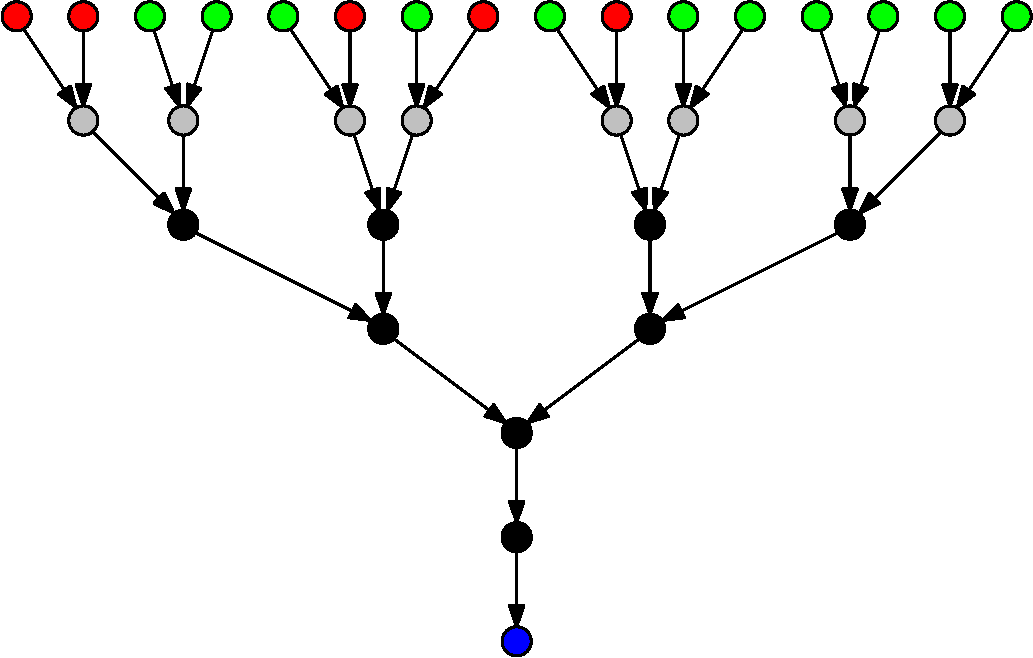
\includegraphics[scale=0.2]{topo-tree-evil-5-good-0-producer-gw}
  \caption{Small-scale binary tree topology}
  \label{fig:small-scale}
\end{figure}

% in 10 independent runs of each simulation, where we randomized position of the adversaries along the legitimate users.   In all runs, the total number of legitimate and malicious uses were fixed, meaning that when we increase number of attackers, we decrease the number of legitimate users.   

\subsubsection{Effectiveness of the three mitigation algorithms}

%The first set of experiments aims to evaluate reaction of the network and Interest flooding attack mitigation methods mechanisms under a moderate-level DDoS attack.
%For this purpose, we simulated four different network scenarios, in which all routers implements the same attack mitigation algorithm, either token bucket with per interface fairness, satisfaction-based Interest acceptance, or satisfaction-based pushback (Section~\ref{sec:design}).

Our goal is to compare the effectiveness of each mitigation method and quantify the percentage of Interests satisfied for all legitimate users while the network is under attack. For each mitigation algorithm, we perform ten independent simulation runs, where we randomly choose 7 client nodes to represent adversaries while the remaining 9 client nodes represent legitimate users. In each run we simulate a 10-minute attack window (total simulation time was 30 minutes, with attack starting at the 10-minute mark). We plot the minimum and maximum range for observed Interest satisfaction percentages for all legitimate users aggregated across the 10 simulation runs as a function of time for each mitigation algorithm in Fig.~\ref{fig:small-scale attack progress}. Token bucket with per-interface fair queuing performs the worst, while satisfaction-based pushback performs the best, with almost a 100\%  satisfied Interests for all legitimate users.

%A short and simplistic summary of the results is that the first two attack mitigation methods do not work at all, and the last two are working quite good.

\begin{figure}[t]
  \centering
  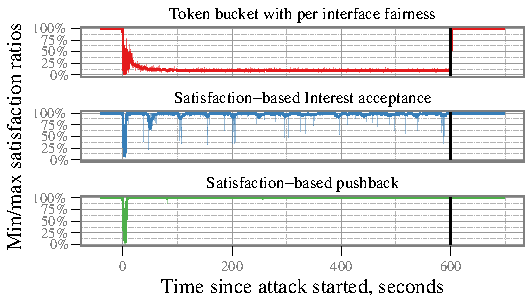
\includegraphics[scale=0.8]{paper-topo-tree/tree-good-0-producer-gw}
  \caption{Interest satisfaction ratio as a function of time for binary-tree topology with 7 attackers and 9 legitimate users}
  \label{fig:small-scale attack progress}
\end{figure}

%\paragraph{\textbf{Simple token bucket}}

%{\color{red}Alex: should this discussion be removed or we still want to keep it (as it is referenced later and potentially before)}

%Let us take a deeper look on what is happening with the simple token bucket algorithm.
%Essentially, we observe an extremely successful denial of service attack, where attackers almost completely shut down legitimate users from the Data producer (using a relatively small amount of Interests, as token bucket restricts the number of forwarded Intersets!).
%This ``success'' can be explained using a simplistic example, illustrated on Fig.~\ref{fig:three router example}, where each router has only one token for Interest forwarding.
%In this example we assume that both the legitimate user and the adversary send Interests in about the same time.
%
%\begin{figure}[t]
%  \centering
%  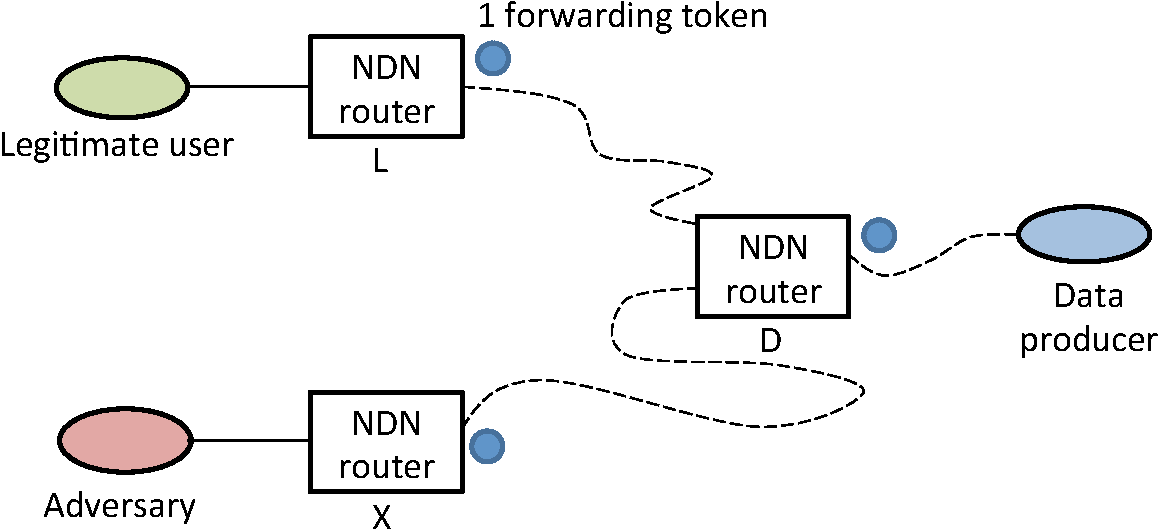
\includegraphics[scale=0.3]{physical-limits-sync-problem}
%  \caption{Three-router topology, with one legitimate and one malicious user}
%  \label{fig:three router example}
%\end{figure}
%
%Both router L and router X will forward the Interests, as both of them have a free token available.
%At router A, two cases are possible, either of Interests can arrive first, resulting in a quite different effects.
%When legitimate Interest arrives first, then there are no problem. 
%Router A will capture the token, forward the Interest, which will be quickly satisfied, releasing the token for future uses.
%In the mean time, malicious Interest will be dropped at router A, and router X will release the hold for the token in one second (i.e., after the maximum time Interests are admitted), enabling a new round of competition for router A's resources.
%
%In the case when malicious Interest is sent a little bit earlier, then router A will forward malicious Interests, dropping a legitimate one, and causing ``lock out'' for one second.
%In the instant when the token gets released at router X, an adversary is able to push new Interest towards router A, which may arrive in the exact time A's token gets released (assuming an idealistic environment).
%As a result, the adversary recaptures router A's token and extends the ``lock out'' for another second, denying service to the legitimate user without sending any massive numbers of Interests.

\paragraph{\textbf{Token bucket with per interface fairness}}

We observe a successful denial of service attack, where 40\% attackers succeed in significantly shutting down the remaining 60\% legitimate users - a mere 15\% of their Interests are satisfied by Data from the producer. Contrary to expectations, the 60\% legitimate users do not receive at least 60\% of network resources. As described in the previous section, the key limitation of this algorithm is that it still admits Interests from attackers, a good percentage of which traverse all the way to the data producer. Significantly reducing the number of Interests accepted from attackers is fundamental for improving the effectiveness of any mitigation algorithm. 

%The described problem arises from the clocking effect and can be solved in a number different ways.
%Augmenting token bucket algorithms with per-interface fair queueing allows us to eliminate the clocking effect. 
%That is, in the second case when router A releases the token after the first ``lock out'' period, it will immediately process previously enqueued Interests from the legitimate user.
%However, because the Interest time out (``lock out'' time) is most likely be larger than the time to actually fetch the Data, an adversary is still able to ``unfairly'' deny service to good guys.
%Ideally, if there are only 40\% of compromised users, the rest good users should get at least 60\% of network resources, which is not true as can be seen on Fig.~\ref{fig:small-scale attack progress}.
%We expect that reducing the maximum hold time for Interests (e.g., to an order of average RTT) would improve overall performance for legitimate users, with negative effect of requiring extra complexity for Intersets processing.

\paragraph{\textbf{Satisfaction-based Interest acceptance}}

The effectiveness of this algorithm stems from the fact that routers do not admit malicious Interests into the network, thereby ensuring availability of network resources for serving legitimate users. The observed periodic dips in the Interest satisfaction ratios of legitimate users in Fig.~\ref{fig:small-scale attack progress} is a direct result of Interest satisfaction rate statistics decaying with time. The 50-second period approximately corresponds to the selected exponential decaying parameter $\alpha=e^{−1.0/30.0}$, which decays statistics to $1/e$ of the initial value that ranges from 30~seconds to 50~seconds. 
%The primary reason that such minimum peaks exist is the fact that 
When Interests from attackers start to get readmitted, they cause degradation of statistics on routers close to the producer (i.e., routers that observe traffic mix from legitimate and malicious users). Consequently, this degradation reduces the probability of legitimate Interests getting through (see Section~\ref{sec:probabilistic}) until malicious Interests are ``pushed back'' to the edge.

%When routers more intelligently process incoming Interests (i.e., based on the incoming interface statistics), the Interest flooding attack becomes virtually ineffective.
%That is, malicious Interests are simply not getting admitted to the network, not being able to create much service disturbance for the legitimate users.

\paragraph{\textbf{Satisfaction-based pushback}}

This mitigation algorithm is able to effectively shut down attackers and ensure that almost all of the Interests from legitimate users are satisfied. 
%The only potential problem with the satisfaction-based pushback algorithm is that it features 
We observe a  sharp dip in the satisfaction ratio curve at the start of the attack.  It takes a few seconds for all routers to be fully aware of the attack, which happens when malicious Interests start to time out and explicit Interest limit announcements succeed in containing malicious Interests close to the attacker. Till then, the network for a short period of time (under 10~seconds for all simulation runs), fails to provide 100\% service for legitimate users. Once the malicious Interests are effectively shut down, all Interests from legitimate users are satisfied. Unlike the satisfaction-based Interest acceptance scenario, we do not observe any periodic dips in the satisfaction curve, as the pushback algorithm effectively guarantees that once an Interest is admitted, it will almost certainly be routed to the data producer.

\subsubsection{Network reaction with to varying number of attackers}

Our next goal is to study the effectiveness of our mitigation algorithms as a function of increasing adversaries in the network.
To this end, we vary the percentage of attackers in the topology from 6\% to over 50\%. Since the total number of end users in the topology is constant, as the number of attackers increases, the number of legitimate users decreases. All other parameters and experimental set-up are similar to the previous experiment. As before, for each mitigation algorithm, we perform ten independent simulation runs.
%The second set of conducted experiments was aimed to answer the question of the effect and quality of the Interest flooding attack mitigation algorithm under different attack volume.
%To do this, for each algorithm we varied the number of adversary nodes in the topology, keeping the total number of client nodes constant: 1 attacker and 15 legitimate users, 3 attackers and 13 legitimate users, etc.

%Since at this point the overall attack dynamics of all the attack mitigation algorithms is relatively clear, 
% In other words, each point captured in the box plot graph corresponds to 1-second averaged satisfaction ratio for a user in an individual simulation run.

\begin{figure}[htbp]
  \centering
  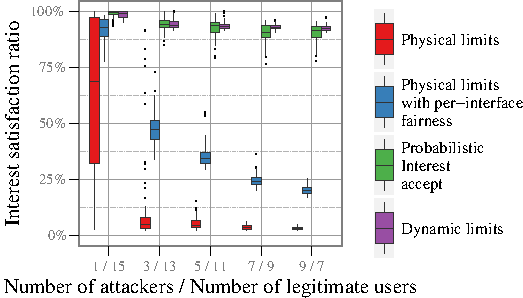
\includegraphics[scale=0.8]{paper-topo-tree/tree-good-0-producer-gw-avg-1-min}
  \caption{Average Interest satisfaction ratios for the first minute of the experiment as a function of increasing attackers in the network}
  \label{fig:small-scale-topo boxplot}
\end{figure}

In Fig.\ref{fig:small-scale-topo boxplot} we present  the Interest satisfaction ratio for legitimate users aggregated over the 10 simulation runs for the first minute of the attack. The results are as expected --- for all three mitigation algorithms, as the percentage of attackers in the network increases, the lower is the Interest satisfaction ratio for legitimate users.
In the case of token bucket with per-interface fairness algorithm, just 3 attackers can halve the quality of service for the remaining 13 legitimate users. While both intelligent attack mitigation algorithms also show a decline in service quality as the percentage of attackers increases, this decline is much more gradual. In the case of satisfaction-based pushback algorithm, over 90\% of Interests from legitimate users are satisfied even when over 50\% of the users are malicious.  
 


% \begin{figure}[htbp]
%   \centering
%   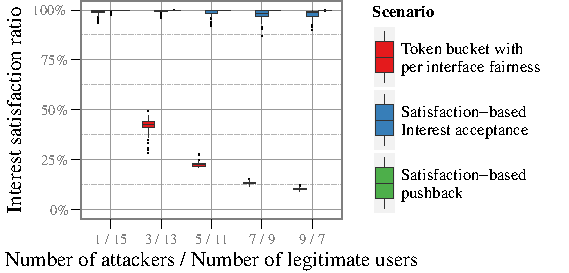
\includegraphics[scale=0.9]{tree-topo-var-evils-max-consumers-30mins/tree-good-0-producer-gw-avg-1-min-after-1-min}
%   \caption{Average consumer Interest satisfaction ratios (second minute)}
%   \label{fig:small-scale-topo 2}
% \end{figure}


%%% Local Variables: 
%%% mode: latex
%%% TeX-master: "paper"
%%% End: 
